\documentclass[a4paper, 12pt]{report}
\usepackage{graphicx}
\usepackage[french]{babel}
\usepackage{caption}
\usepackage[utf8]{inputenc}
\usepackage[T1]{fontenc}
\usepackage{multirow}
\usepackage{listings}
\usepackage{float}
\usepackage{url}
\usepackage[french]{algorithm}
\usepackage{style/myalgorithm}
\usepackage{amsmath,amsfonts,amssymb}
\newcommand{\fBm}{\emph{fBm}~}
\newcommand{\etal}{\emph{et al.}~}
\newcommand{\glAd}{\emph{GL4D}~}
\newcommand{\apiopengl}{API OpenGL\textsuperscript{\textregistered}~}
\newcommand{\opengl}{OpenGL\textsuperscript{\textregistered}~}
\newcommand{\opengles}{OpenGL\textsuperscript{\textregistered}ES~}
\newcommand{\clang}{langage \texttt{C}}
\newcommand{\codesource}{\textsc{Code source}~}
\floatstyle{ruled}
\newfloat{programslist}{htbp}{locs}
\newcommand{\listofprograms}{\listof{programslist}{Liste des codes source}}
\newcounter{program}[subsection]
\renewcommand{\theprogram}{\arabic{chapter}.\arabic{program}}

\newenvironment{program}[1]{
  \if\relax\detokenize{#1}\relax
  \gdef\mycaption{\relax}
  \else
  \gdef\mycaption{#1}
  \fi
  \refstepcounter{program}
  \addcontentsline{locs}{section}{#1}
  \footnotesize
}{
  \begin{description}
    \item[\codesource \theprogram]--~\mycaption
  \end{description}
}

\begin{document}
\begin{titlepage}
  \begin{center}
    \begin{tabular*}{\textwidth}{l@{\extracolsep{\fill}}r}
      
\includegraphics[height=1.5cm]{images/m2ise.png}
    \end{tabular*}
    \small 
    \rule{\textwidth}{.5pt}~\\
    \large 
    \textsc{Université Paris 8 - Vincennes à Saint-Denis}\vspace{0.5cm}\\
    \textbf{Master Informatique des Systèmes Embarqués}\vspace{3.0cm}\\
    \Large
    \textbf{Memoire de projet tuteuré}\vspace{1.5cm}\\
    \large
    \textbf{Fakhri \textsc{YAHIAOUI} - Roman \textsc{BOURSIER}}\vspace{1.5cm}\\
    Date de soutenance : le 09/06/2020\vspace{1.75cm}\\
  \end{center}\vspace{1.5cm}~\\
  \begin{tabular}{ll}
    \hspace{-0.45cm}Tuteur -- Université~:~&~Farès \textsc{BELHADJ}\\
  \end{tabular}
\end{titlepage}
\chapter*{Résumé}
\markboth{\sc Résumé}{}
\addcontentsline{toc}{chapter}{Résumé} 

A faire en dernier ...


\chapter*{Remerciements}
\markboth{\sc Remerciements}{}
\addcontentsline{toc}{chapter}{Remerciements} 

Idem ...

%% Table des matières
\tableofcontents

\chapter*{Introduction}
\markboth{\sc Introduction}{}
\addcontentsline{toc}{chapter}{Introduction}


Dans le cadre de notre projet de fin d'études, nous souhaitons utiliser un modèle de Deep Learning, afin de produire un moteur de rendu capable d’adopter une stylisation « type » tel que la peinture chinoise. Dans un premier temps, il s’agira de proposer un modèle d’abstraction des peintures sélectionnées comme base d’apprentissage et d’utiliser le couple « peinture originale » / « abstraction » pour l’entraînement. Par la suite, un moteur de rendu d’abstractions sera connecté au réseau profond qui produira une peinture sur la base de l’abstraction.

Le modèle généré devra d'une part adopter la stylisation retenue mais aussi interpréter l'abstraction d'origine.

\section{Problématique}

La "traduction image-image" (Image-to-image translation) permet d'apprendre le mapping entre une image d'entrée et de sortie. En figure \ref{fig-pix2pix}, nous testons la génération d'un paysage à partir d'un croquis simple. En figure \ref{fig-pix2pix-fail}, c'est un échec.

\begin{center}
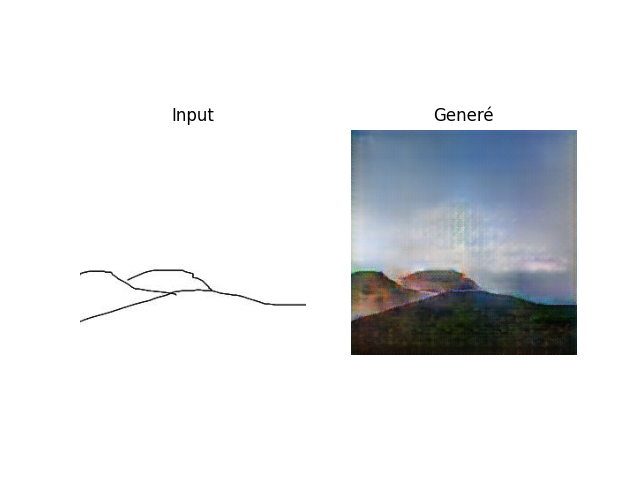
\includegraphics[width=0.7\linewidth]{images/pix2pix-t1.png}
\captionof{figure}{Test du framework pix2pix \cite{DBLP:journals/corr/IsolaZZE16} sur notre dataset composé de photos de paysages, labellisées en appliquant un filtre Canny \cite{4767851} sur chacune d'elles.}
\label{fig-pix2pix}
\end{center}

\begin{center}
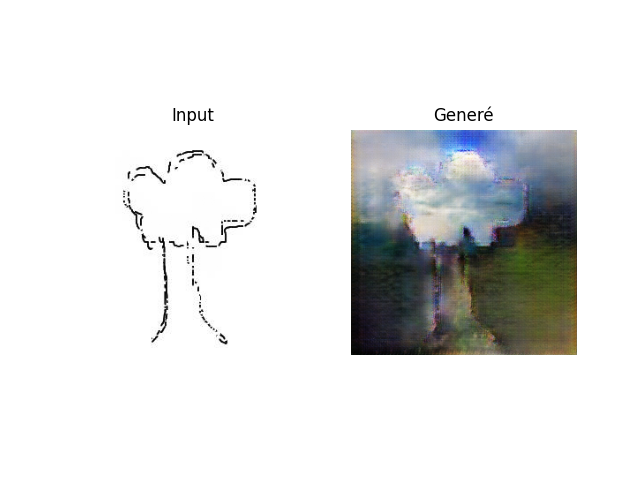
\includegraphics[width=0.7\linewidth]{images/pix2pix-fail.png}
\captionof{figure}{Utilisation du même modèle avec une abstraction d'arbre}
\label{fig-pix2pix-fail}
\end{center}

Comme évoqué dans \cite{DBLP:journals/corr/abs-1805-00247} les algorithmes du type "traduction image-image" se basent essentiellement sur la corrélation d'une image à l'autre, et relève d'un apprentissage supervisé. Le rendu en figure \ref{fig-pix2pix-fail} s'explique par la nature du dataset et par la distance importante qui sépare une abstraction d'une photo. 

En figure \ref{fig-croquis} nous avons demandé à plusieurs personnes de dessiner un paysage composé de montagnes et d'arbres, éléments courants de la peinture chinoise. Ces dessins sont des abstractions, que nous souhaitons traduire en peintures chinoises.

\begin{center}
  \centering
  \begin{tabular}{ccc}
    \includegraphics[angle=90, height=0.15\textheight]{images/croquis_1.jpg}&
    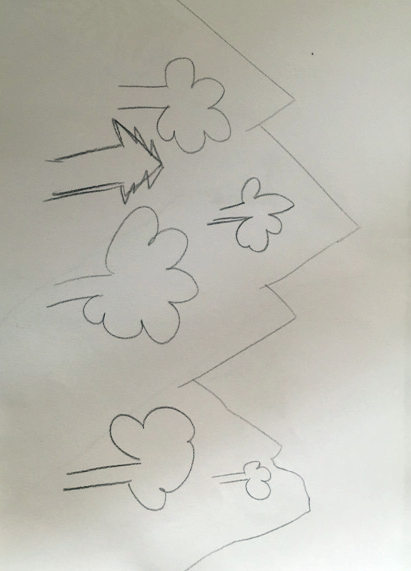
\includegraphics[angle=90, height=0.15\textheight]{images/croquis_2.jpg}&
    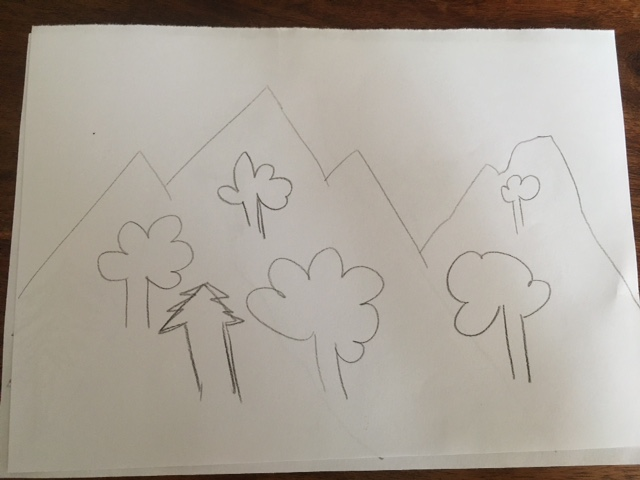
\includegraphics[angle=90, height=0.15\textheight]{images/croquis_4.jpg}\\
    (a)&(b)&(c)
  \end{tabular}
  \captionof{figure}{Dessin de paysages réalisés par des personnes différentes. On note que les niveaux d'informations sont plus ou moins élevés. Le dessin (b) est très abstrait tandis que nous observons plus de détails pour (a) .\label{fig-croquis}}
\end{center}



\chapter{Etat de l'art}
 
Nous présentons dans un premier temps les GANs qui sont au coeur de notre problématique. En un second lieu, nous étudions différents modèles existants basés sur les GANs conditionnels. Nous évoquons aussi, de manière plus succincte, des travaux liés à notre sujet mais n'utilisant pas les réseaux de neurones afin de pouvoir identifier les avantages et inconvénients des deux approches. Nous terminons par une liste des datasets utiles à notre sujet.


\section{Généralités sur les GANs}

"Les GANs (en anglais generative adversarial networks) sont une classe d'algorithmes d'apprentissage non-supervisé. Ces algorithmes ont été introduits dès 2014 par Goodfellow et permettent de générer des images avec un fort degré de réalisme." \cite{wiki:Reseaux-antagonistes-generatifs}

Un générateur fabrique des données et les soumet au discriminateur dont le but est d'évaluer leurs degrés de crédibilité. 

Le générateur $G(z, \theta_{1})$ représente un réseau de neurones capable de mapper du bruit $z$ vers l'espace désiré $x$. Le discriminateur $D(z, \theta_{2})$ retourne la probabilité dans l'intervalle $[0,1]$ que $x$ vient du dataset original. $\theta_{i}$ représente les poids définis par chacun des modèles. Le générateur tente de maximiser la probabilité que les données $x$, soient classifiées comme appartenant au dataset d'origine et inversement, le discriminateur minimise la probabilité que de fausses images appartiennent au dataset d'origine.

Il existe aujourd'hui une très grande variété de travaux de recherche basés sur les GANs (BCGAN, AmbientGAN, ORGAN, Perceptual GAN). Le dépôt "The GANs Zoo" \cite{hindupuravinash} référençait déjà en 2018 plus de 502 noms de GANs différents !


\section{CGANs et traduction d'image}

Les GANs conditionnels ajoutent une information supplémentaire $y$, partagée par le discriminateur et le générateur. Grâce aux cGANs il est possible de générer des images réalistes basées sur des labels de classes, des textes ou des images.

\subsection{Pix2Pix}
\cite{DBLP:journals/corr/GatysEB15a} nous montre en quoi les cGANs peuvent permettre de résoudre efficacement les problèmes de traductions d'images et propose un framework applicable à n'importe quel domaine.

\subsection{GauGan}
\cite{DBLP:journals/corr/abs-1903-07291} permet de générer des paysages réalistes basés sur des masques de segmentation sémantiques. Les auteurs introduisent la "normalisation conditionnel" ou "adaptative", permettant de prendre en compte notamment les informations spatiales.
Les couches de normalisations ont tendance à faire perdre de l'information contenu dans les masques sémantiques d'entrées car ils ne dépendent pas de données externes.

\begin{center}
  \centering
  \begin{tabular}{cc}
    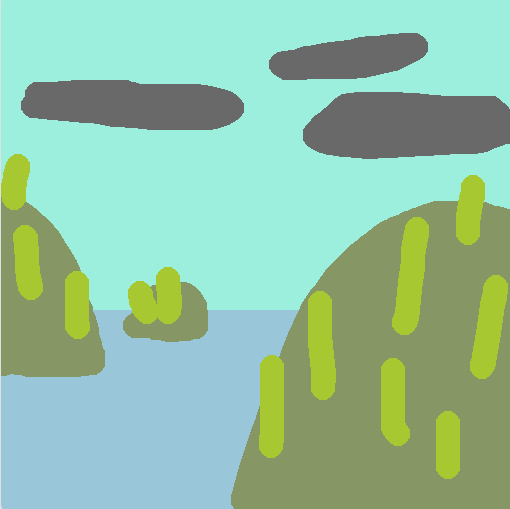
\includegraphics[height=0.15\textheight]{images/test-gaugan-sm.jpg}&
    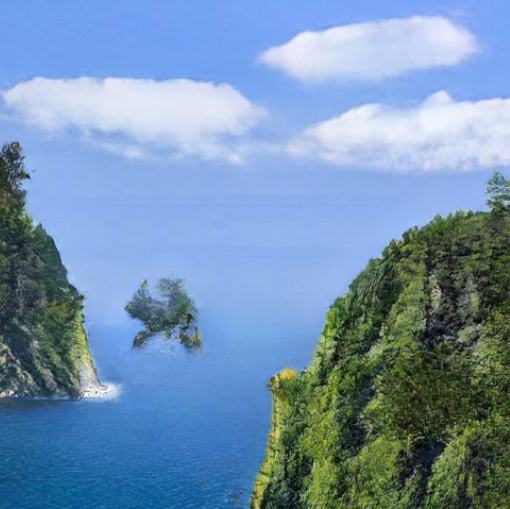
\includegraphics[height=0.15\textheight]{images/test-gaugan.jpg}\\
    (a) Input - masques de segmentation sémantiques &(b) Output
  \end{tabular}
  \captionof{figure}{Test de rendu de paysage à partir de l'application Gaugan : http://nvidia-research-mingyuliu.com/gaugan/\label{fig-gaugan}}
\end{center}

\subsection{CycleGan}
CycleGan \cite{CycleGAN2017}, présente une approche pour la traduction d'une image d'un domaine source vers un domaine cible lorsque le dataset n'est pas apparié. \\

Le modèle possède deux générateurs $G:X\to Y$ et un second $F:Y\to X$ ainsi que deux discriminateurs $D_Y$ and $D_X$

Les auteurs nous expliquent que si nous pouvons passer du domaine $X$ vers le domaine $Y$ et vice-versa, alors le résultat final devrait être identique à l'entrée initiale $X$.

\subsection{Transfert de style neuronal} 
Introduit par Leon A. Gatys \cite{DBLP:journals/corr/GatysEB15a} le TDN consiste à transférer un style à partir d'une image de référence vers une image de contenu. L'objectif est de transformer l'image d'entrée (bruit) en minimisant la distance avec l'image de contenu et avec l'image de style. On obtient alors par rétropropagation, une image qui correspond au contenu de l'image d'origine et au style souhaitée.

L'avantage de cette technique est qu'elle ne nécessite pas de dataset, seules deux images sont nécessaires.

\begin{center}
  \centering
  \begin{tabular}{ccc}
    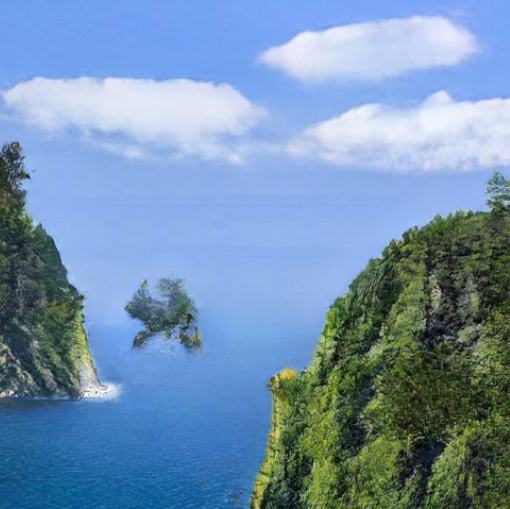
\includegraphics[height=0.15\textheight]{images/test-gaugan.jpg}&
    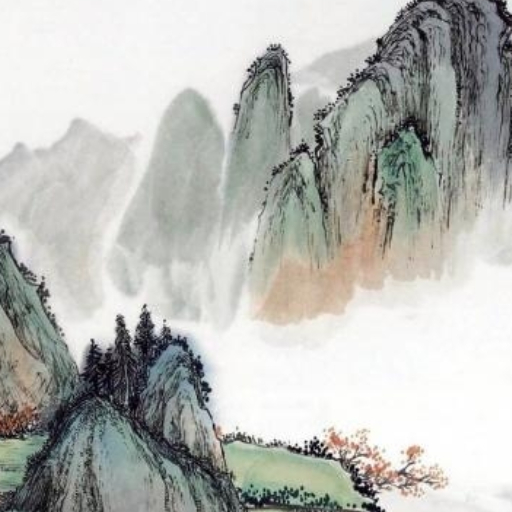
\includegraphics[height=0.15\textheight]{images/transfert-ds.jpg}&
    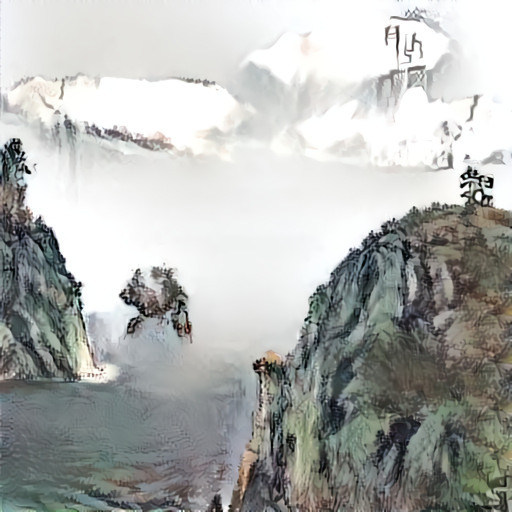
\includegraphics[height=0.15\textheight]{images/gaugan-tds.jpg}\\
    (a) Image de contenu & (b) Image de style &(c) Résultat
  \end{tabular}
  \captionof{figure}{Test de transfert de style réalisé à partir de la figure \ref{fig-gaugan}\label{fig-transfert-de-style}(b)}
\end{center}


\subsection{Learning to Sketch} 
\cite{DBLP:journals/corr/abs-1805-00247} présente une méthode permettant de transformer une photo en croquis, en essayant d'imiter la façon de faire d'un humain. Le modèle est capable de réaliser le croquis séquentiellement, c'est-à-dire trait par trait. Les auteurs proposent de résoudre le problème des styles subjectifs et variés des dessins fait à la main en utilisant un modèle hybride supervisé/non-supervisé. L'objectif étant de palier "au signal de supervision faible et bruyante" induit par l'écart important entre un croquis et sa photo correspondante. \\

L'architecture est décomposé en 4 sous-modèles contenants chacun leurs propres sous-réseaux d'encodeurs et de décodeurs. Deux réseaux supervisés traduisent respectivement une photo en croquis $D(E(photo))\to sketch$ et un croquis en photo $(D(E(sketch))\to photo)$ . Deux autres réseaux non-supervisés se chargent de la reconstruction. $D(E(photo))\to photo$ et $D(E(sketch))\to sketch$  \\


\subsection{Sketching: Inferring Contour Drawings from Images}
\cite{DBLP:journals/corr/abs-1901-00542} propose une nouvelle approche concernant la détection des contours dans une image. L'article montre que les solutions traditionnelles comme Canny \cite{4767851} , captent uniquement les signaux de haute fréquence dans l’image sans la comprendre. Les auteurs ont collecté un dataset de 5000 pairs "croquis humain/photos", crée manuellement via la plateforme de crowdsourcing "Amazon Mechanical Turk". En effet aucun dataset existant ne convenait (nombre d'éléments dans l'image, limites internes manquantes, le contenu non reconnaissable, les zones ombrées vides etc ..).

Ce modèle également du type "traduction image-image", permet d'avoir plusieurs labels différents pour la même photo, donc plusieurs interprétations différentes.

\begin{center}
  \centering
  \begin{tabular}{cc}
    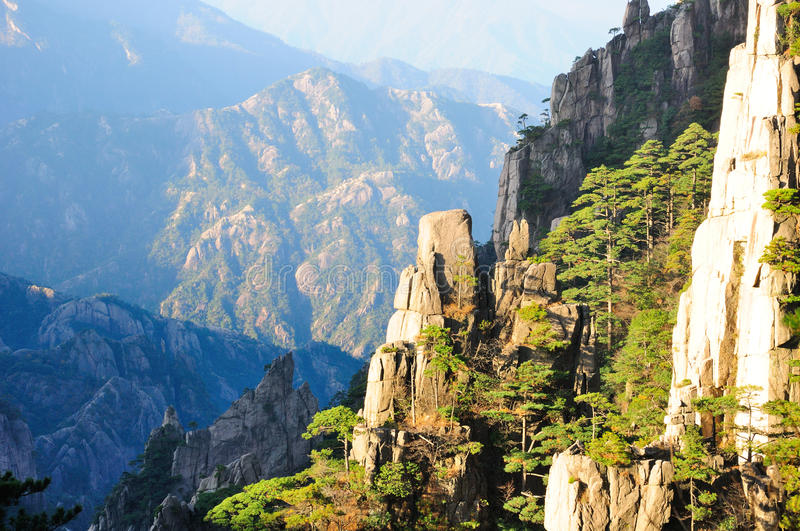
\includegraphics[height=0.15\textheight]{images/sketching-input.jpg}&
    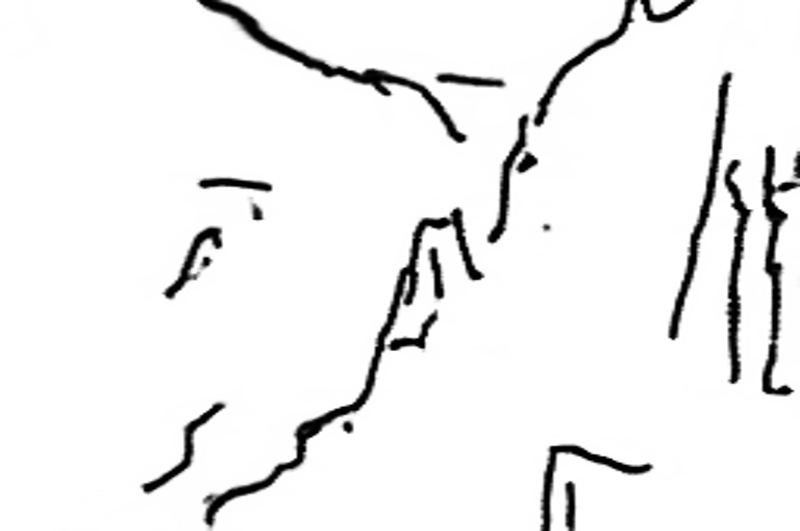
\includegraphics[height=0.15\textheight]{images/sketchy2.png}\\
    (a) Input &(b) Output
  \end{tabular}
  \captionof{figure}{Test du modèle pré-entraîné sur une photo de paysage\label{fig-gaugan}}
\end{center}




\chapter{Proposition de solution}



\section{Datasets}

Malgrè nos recherches, nous n'avons pas pu trouver de dataset correspondant exactement à nos besoins, c'est-à-dire des paires d'abstraction/peinture chinoise.Pour les croquis, les plus grosses bases existantes sont TU-Berlin \cite{eitz2012hdhso}, Sketchy \cite{sketchy2016} et Quickdraw. Après plusieurs essais, nous avons décidé d'abandonner leurs utilisations car il s'agit le plus souvent d'objets isolés et non appairés à une image réaliste. Pour la peinture chinoise, nous avons récupéré un premier dataset de 5000 images (\cite{ychen93}) et scrappés des plateformes comme google/baidu et pinterest. 


Au final notre dataset est composé de 624 peintures de paysage chinoises réparties en 90/10 (90\% des images destinées à l'entraînement et 10\% pour les tests). Nous les avons ensuite réduites essentiellement pour des raisons de temps et d'apprentissage trop long. Chaque image sera par la suite redimensionnée et recadrée au format 256x256.


\section{Modèle}
Nous proposons de diviser l'apprentissage en deux étapes. La première consiste à traduire un croquis en dessin détaillé et la seconde d'un dessin détaillé vers la peinture. Notre proposition se base sur deux cGan de type "image-image", entraîné sur deux datasets appairées.


L'implémentation utilise le framework Keras et se base sur l'architecture pix2pix[].

\begin{center}
  \centering
    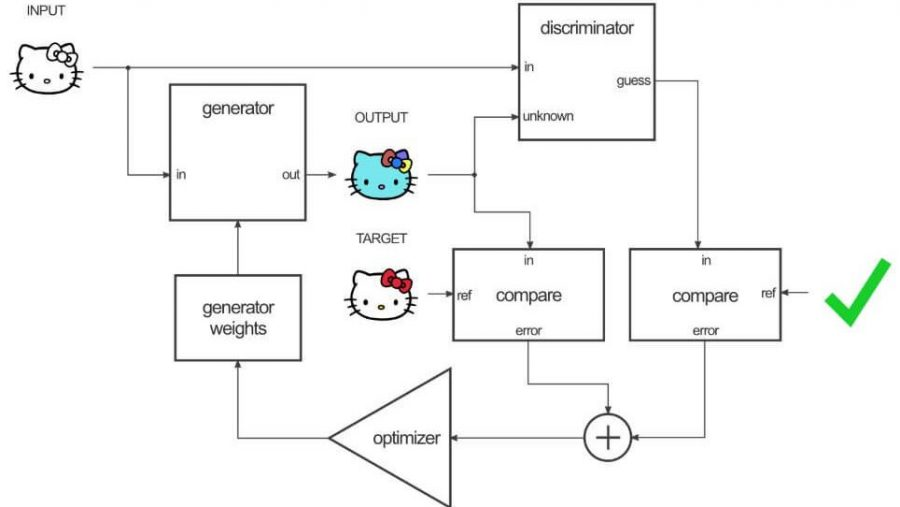
\includegraphics[width=0.8\linewidth]{images/pix2pix.jpg}
  \captionof{figure}{Pix2pix \ref{fig-gaugan}\label{fig-transfert-de-style}(b)}
\end{center}




\section{Abstraction vers photo}
Au départ, nous avosn réalisé directement un pix2pix sur le dataset croquis/photos. Cependant, nous avons remarqué que les résultats n'étaient pas celles qu'on espéraient (voir figure \ref{pix2pix-color}). Pour un dessin fait main nous pouvons constater que le résultat est un peu brouillon tandis qu'avec une image en entrée où le filtre Canny est appliqué le résultat est plus satisfaisant (voir figure \ref{pix2pix-canny-color})

\begin{figure}[!h]
\centering 
\begin{minipage}{0.45\textwidth}
\centering
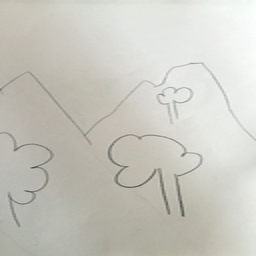
\includegraphics[scale=0.5]{images/croquis_2_real_A.png}
\\Croquis
\\
\end{minipage}
\begin{minipage}{0.45\textwidth}
\centering
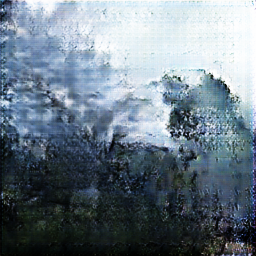
\includegraphics[scale=0.5]{images/croquis_2_fake_B.png}
\\Résultat en couleur
\end{minipage}
\caption{\centering Résultat pix2pix croquis en entrée.}
\label{pix2pix-color}
\end{figure}

\begin{figure}[!h]
\centering 
\begin{minipage}{0.45\textwidth}
\centering
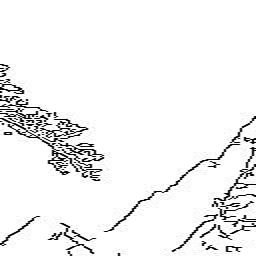
\includegraphics[scale=0.5]{images/roro-1_real_A.png}
\\Image avec filtre Canny
\\
\end{minipage}
\begin{minipage}{0.45\textwidth}
\centering
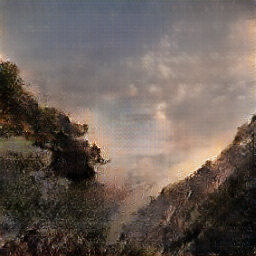
\includegraphics[scale=0.5]{images/roro-1_fake_B.png}
\\Résultat en couleur
\end{minipage}
\caption{\centering Résultat pix2pix avec image Canny en entrée.}
\label{pix2pix-canny-color}
\end{figure}
\newpage
C'est pour cette raison, qu'après plusieurs expériences décevantes, nous avons choisi d'utiliser un algorithme de détection de bord nommé "holistically-nested edge detection" (HED) pour traduire nos peintures en dessins détaillées. Cette solution basée sur un modèle d'apprentissage profond permet de résoudre l’ambiguïté liée à la détection des contours et des objets.

A partir de cette sortie notre but est d'extraire le maximum d’éléments de l'image en ne gardant que les caractéristiques les plus représentatives. Nous avons testé plusieurs méthodes.

[Todo inclure les tests]

Après essais sur le modèle d'apprentissage, il s'avère que la labellisation manuelle reste dans notre cas le plus satisfaisant.

Nous pensons néanmoins que deux méthodes auraient mérité d'être approfondies, celle la segmentation ainsi que l’algorithme de Ramer–Douglas–Peucker. Dans les deux cas, l'avantage majeur est d'épargner la labellisation manuelle.


\section{Photo vers peinture}
Afin de réaliser la peinture chinoise à partir de la photo, nous avons pensé directement au cyclegan. Lors de nos recherches, nous avons pu constater des exemples de cyclegan générant des peintures de style monet à partir d'une photo. \\
N'ayant pas de photos de paysage qui ressemblent aux paysage dans les peintures chinoises, nous avons tout de même réussi à appliquer le style propre aux peintures chinoise sur ces photos.\\
De plus, pour plus de rapidité nous avons réduit le nombre de dataset donc il est probable que ça a eu un impact sur le résultat. Aussi, en raison de la durée limitée sur google colab l'entraînement n'a pas pu être fini (voir les figures ci-dessous pour les résultats). 


\begin{figure}[!h]
\centering 
\begin{minipage}{0.45\textwidth}
\centering
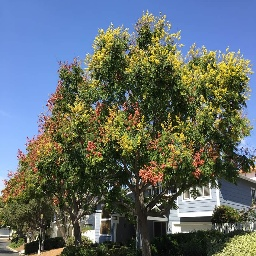
\includegraphics[scale=0.5]{images/cyclegan_real_A.png}
\\Photo donné au cyclegan
\\
\end{minipage}
\begin{minipage}{0.45\textwidth}
\centering
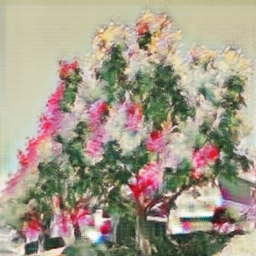
\includegraphics[scale=0.5]{images/cyclegan_fake_B.png}
\\Photo avec peinture chinoise appliquée
\end{minipage}
\caption{\centering Résultat cyclegan de la photo à la peinture chinoise.}
\label{cyclegan-result}
\end{figure}

\begin{figure}[!h]
\centering 
\begin{minipage}{0.45\textwidth}
\centering
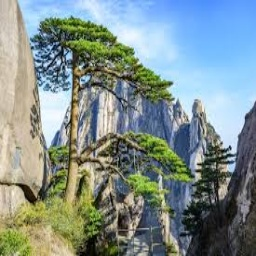
\includegraphics[scale=0.5]{images/cyclegan_real_A-2.png}
\\Photo donné au cyclegan
\\
\end{minipage}
\begin{minipage}{0.45\textwidth}
\centering
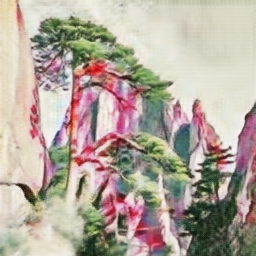
\includegraphics[scale=0.5]{images/cyclegan_fake_B-2.png}
\\Photo avec peinture chinoise appliquée
\end{minipage}
\caption{\centering Résultat cyclegan de la photo à la peinture chinoise.}
\label{cyclegan-result-fail}
\end{figure}


Comme on peut le constater, malgré le modèle non fini, à la figure \ref{cyclegan-result} le résultat est assez réussi. Cepedant on peux remarquer que dans la figure \ref{cyclegan-result-fail} les même couches de peintures sont appliqué mais qui donne un résultat peu convaincant. \\
Ce résultat est probablement dû au fait que l'entraînement n'est pas fini (ça s'est arrêté à la 45ème epoch sur 200).

\chapter{Résultats}
- Graphique temps d'apprentissages (CPU collab/pc perso) / exécutions\\
- Plot d'images

\begin{figure}[!h]
\centering
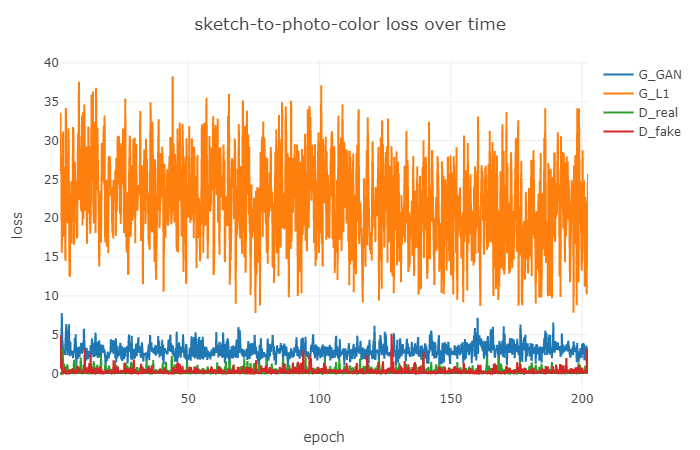
\includegraphics[scale=0.5]{images/plot-pix2pix.png}
\end{figure}

\begin{figure}[!h]
\centering
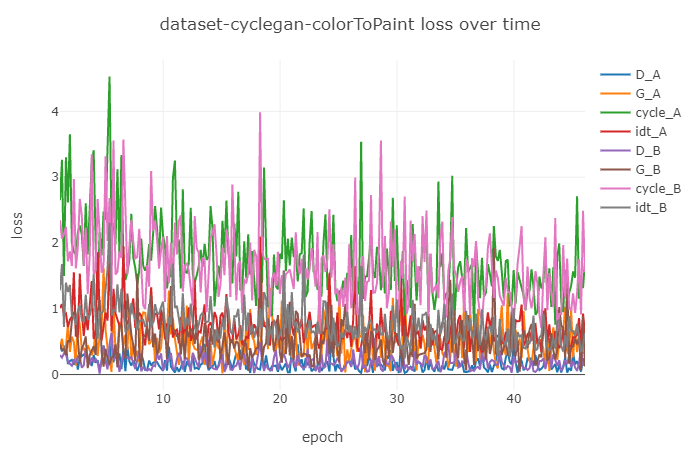
\includegraphics[scale=0.5]{images/plot-cyclegan.png}
\end{figure}

\chapter{Conclusion et Perspectives\label{chap-conclusion}}

Comme nous l'avons évoqué dans la section état de l'art, il est possible d'appliquer efficacement un style donné à une image, mais pour que le rendu soit crédible, il faut que l'entrée provienne d'une image réaliste. Notre principale difficulté était donc de transformer une abstraction en dessins réaliste. Les résultats présentés montrent que des modèles comme pix2pix permettent de réaliser ce transfert à condition d'avoir un dataset spécialisé (paysage)et appairé. Ainsi plus y a de variation et de disparité dans le dataset, moins la prédiction sera convaincante.

Par ailleurs, nous savons que les RCNNs, grâce aux couches de convolutions, sont capables de détecter les caractéristiques visuelles communes d'un ensemble d'images. Comme le prouve ce travail : https://medium.com/artists-and-machine-intelligence/perception-engines-8a46bc598d57, il est peut-être possible de générer une représentation abstraite de nos peintures en utilisant ce principe. Il serait alors théoriquement possible d'obtenir des paires abstractions/peintures, permettant l'entraînement d'un cGAN type "traduction image-image". 

Les résultats pourraient être améliorés en augmentant le nombre d'éléments dans le dataset ainsi que le nombre d'epochs.


\bibliographystyle{alpha}
\bibliography{memoire}
\end{document}
